\section{Method}
\label{sec:method}
\subsection{Algorithm}
The core of modelling current-reinforced random walks is that there are sources, sinks, nodes, particles and edges all organised within a graph representing a network. The fundamental idea is that sources send out information, sinks collect information and particles represent information. Edges are connections between sources, sinks and nodes and represent a path for the information to spread. Sources have a production rate, i.e.\@ the rate at which new particles are being injected into the system. Sinks have a removal rate, i.e.\@ the rate at which particles are being removed from the system. Sources, sinks and nodes can all contain particles. For a system to have a viable solution for a minimised cost function the cumulative production rate of all the sources must be less than or equal to the cumulative removal rate of all the sinks, otherwise no flow equilibrium can be established.

There are some necessary parameters for this model to make sense. These parameters and their analogy in both electrical networks and ant trail networks are shown in Table \ref{tab:parameters}. How these parameters are used in the algorithm is explained in detail in Section \ref{sec:preparation} and \ref{sec:confirmation}.

\begin{table}[H]
\renewcommand{\arraystretch}{1.2}
\centering
\caption{Table shows the necessary parameters for the current-reinforced random walk modelling and their analogy in electrical networks and ant trail networks. The index $i$ denotes that the parameter corresponds to node $i$ and $ij$ denotes that the parameter corresponds to the edge between node $i$ and node $j$.}
\label{tab:parameters}
\begin{tabular}{ c | c | c }                       
	\textbf{Parameter} & \textbf{Electrical network} & \textbf{Ant trails} \\
	\hline
	$l_{ij}$ & length in space & length in space \\
	\hline
	$N_{i}$ & number of electrons & number of ants \\
	\hline	
	$P_{i}$ & potential & density of ants \\	%Could be something like 'current-density of ants'?
	\hline
	$I_{ij}$ & current & flow of ants \\
	\hline
	$\bar{I}_{ij}$ & expected value of current & mean flow of ants \\
	\hline
	$D_{ij}$ & conductivity & pheromone concentration \\
	\hline
	$C_{i}$ & capacitance & total pheromone density \\
	\hline
	$q$ & reinforcement intensity & pheromone drop rate \\
	\hline
	$\lambda$ & conductivity decrease rate & pheromone evaporation rate \\
\end{tabular} 
\end{table}

The underlying algorithm for the current-reinforced random walk can be described by some key steps. At each time step the algorithm can be divided into two parts, one preparation part and one confirmation part. The reason for this is that synchronisation is needed when implementing the algorithm in parallel. This is further explained in Section \ref{sec:parallel}. An outline of this algorithm is shown in Algorithm \ref{alg:outline}.

%The preparation step contains updating of the mean flow $\bar{I}_{ij}$, needed in order to randomise a new number of particles to move from one node to another i.e.\@ the flow $I_{ij}$, and also contains the actual update of the flow $I_{ij}$.
%
%The confirmation step begins with updating the the conductivity $D_{ij}$. The conductivity is needed in order to calculate the new capacitance $C_{i}$. The new number of particles $N_{i}$ within a node is calculated from the previous number of particles and the flow $I_{ij}$ generated in the preparation step. The calculation of $N_{i}$ and $C_{i}$ are not dependent on each other and can be done in any order. The final stage in the confirmation step is the calculation of the potential $P_{i}$, which depends on $C_{i}$ and $N_{i}$. When this is finished the next time step can be started.

{
\vspace{1em}
\begin{algorithm}[H]
Preparation:\\
\ForEach{node}{
	\ForEach{neighbour}{
		calculate mean flow $\bar{I}_{ij}$\;
		randomise new flow $I_{ij}$\;
	}
}
\ \\
Confirmation:\\
\ForEach{node}{
	update number of particles $N_{i}$\;
	\ForEach{neighbour}{
		update conductivity $D_{ij}$\;
	}
 	calculate capacitance $C_{i}$\;
	calculate potential $P_{i}$\;
}
\caption{Outline of the algorithm used in the current-reinforced random walks in \cite{Sumpter}.}
\label{alg:outline}
\end{algorithm}
\vspace{1em}
}

\subsubsection{Preparation}
\label{sec:preparation}
The preparation begins with each node calculating the mean flow $\bar{I}_{ij}$ to each of its neighbours as

\begin{equation}
\bar{I}_{ij} = \frac{(N_i - N_j)D_{ij}}{l_{ij}},
\end{equation}

 \noindent from which it can be seen that the mean flow depends on the conductivity of each edge, $D_{ij}$, which is initialised at and kept at or above some minimal value. The actual flow along the edge $ij$ can then be calculated as

\begin{equation}
I_{ij} = \text{Poi}(|\bar{I}_{ij}|\Delta t).
\end{equation}

In terms of implementation, it is important that nodes that are connected to the same edge agree on the same number of particles to transfer. This is ensured by allowing only the node with a larger number of particles to randomise the value and then both nodes use that value when updating the number of particles. This will also help to ensure that there are never fewer than zero particles at a node, since the number of particles will decrease at the node with the largest number of particles. So, allowing only the nodes with the largest number of particles to randomise the flow means that nodes can be stopped from sending away more nodes than are already at the node. 

The order of randomising the number of particles to move to each neighbouring node is uniformly randomised at each time step for each node. This means that there is no bias in choosing flow calculation order, i.e.\@ no node will always have its number of particles randomised first. When a node has a smaller number of particles than a given neighbour, the node always calculates the flow to that neighbour as zero and then waits for the neighbouring node to tell it how many particles should be moved. After all nodes have calculated and stored $\bar{I}$ and $I$, the preparation step is finished.

\subsubsection{Confirmation}
\label{sec:confirmation}
At the beginning of the confirmation part, all the data regarding how many particles will move along each edge is available. And so each node begins the confirmation by updating the conductivity, which is calculated as

\begin{equation}
D_{ij}(t + \Delta t) = D_{ij}(t) + q|\bar{I}|^\mu - \lambda D_{ij}(t)\Delta t,
\end{equation}

 \noindent where $q$ is the reinforcement intensity caused by per unit flow, $\mu$ is the path maintenance parameter, $\lambda$ is the conductivity decay parameter and $\Delta t$ is the time step. If $\mu$ is set to one the current-reinforced random walk is linear and will converge to the same solution every time. If $\mu$ is set to a value greater than one the current-reinforced random walk becomes non-linear and will not converge to the same solution every time that a system is simulated. In the algorithm's linear state it optimises the path length for each individual path from the sources to the sinks, i.e it minimises the cost function

\begin{equation}
\sum_{j \in \text{Neighbours}(i)} l_{ij} \bar{I}_{ij},
\end{equation}

 \noindent where $l_{ij}$ is the edge length between node $i$ and $j$ and $\bar{I}_{ij}$ is the corresponding mean flow of particles. This means that the algorithm always will find the shortest path through the graph. When utilising the algorithm in its non linear state a combination of path length and path maintenance is optimised. No cost function for the non linear case has analytically yet been found. A proposition for such a cost function is suggested in \cite{Sumpter}. 

After the conductivity is updated the number of particles and the capacitance can be calculated. The new number of particles is calculated as

 \begin{equation}
 N_i(t + \Delta t) = N_i(t) + \sum_{j \in \text{Neighbours}(i)} \left( I_{ji} - I_{ij} \right).
 \end{equation}

 \noindent The capacitance is calculated as 

 \begin{equation}
 C_i = \sum_{j \in \text{Neighbours}(i)} D_{ij}/l_{ij},
 \end{equation}
 
 \noindent and finally the potential is calculated as
 
 \begin{equation}
 P_i = \frac{N_i}{C_i}.
 \end{equation}
 
 \noindent When this is done the time step is finished and the next time step can be started.

\subsection{Implementation and parallelism} 
\label{sec:parallel}
In order to achieve good performance it is important to implement the algorithm within a high performance environment. An ideal programming language for applications with high performance requirements is \texttt{C++}, which gives the programmer good control over optimisations and provides support for low level memory manipulation. It is also a good language for object oriented programming, which makes application design much easier. Other good features of \texttt{C++} is that it has generic and imperative programming features and is also very well suited for implementing parallel applications, both when utilising smaller shared memory models and big scale message passing systems. Since the simulations done in \cite{Sumpter} were implemented serially in Matlab, \texttt{C++} is a very suitable language of choice for significantly increasing the performance and taking the simulations into the parallel realm.

The algorithm shown in Algorithm \ref{alg:outline} can be parallelised in each of the outer loops, with synchronisation after each preparation step and after each confirmation step. The synchronisations are necessary since the update of the conductivity depends on the flow from the neighbouring nodes and since the update of the mean flow depends on the potential of the neighbouring nodes. Therefore, a node and its neighbours must all have done the necessary steps before moving on to the confirmation part. So strictly speaking, global synchronisation is not necessary, i.e.\@ all nodes must not wait for all nodes to finish the preparation part, a node must only wait for its neighbours to finish. However, global synchronisation is much simpler implementation-wise and may not be slower since it avoids complicated synchronisation patterns.

The actual implementation uses OpenMP \cite{openmp} to parallelise the computations, the outer for-loops in Algorithm \ref{alg:outline} are parallelised using the directive \texttt{\#pragma omp parallel} with a \texttt{\#pragma omp barrier} in between them. Each of the for-loops explicitly assigns the nodes within a partition to each core, perfectly matching the nodes assigned to a core with the graph partitions generated by the method described in Section \ref{sec:graph_part}.

\subsection{Graph partitioning}
\label{sec:graph_part}
When utilising multicore systems it is important to minimise cache invalidation, i.e.\@ communication between cores, in order to get good performance. This can be done in numerous ways but when working with graphs a natural way of minimising cache invalidation is to partition the graph. Partitioning the graph must be done in a clever way so that there are as few edges as possible connecting nodes belonging to different cores. A rigorous way of partitioning graphs is presented in \cite{Lasalle}. A schematic view of such a graph partitioning is shown in Figure \ref{fig:partitioning}. Graph partitioning has been studied extensively, hence many softwares for partitioning graphs in good ways have been developed through the years. The particular software used for the graph partitioning in this project is METIS \cite{Lasalle}. 

\begin{figure}
\centering
\begin{subfigure}[b]{0.48\textwidth}
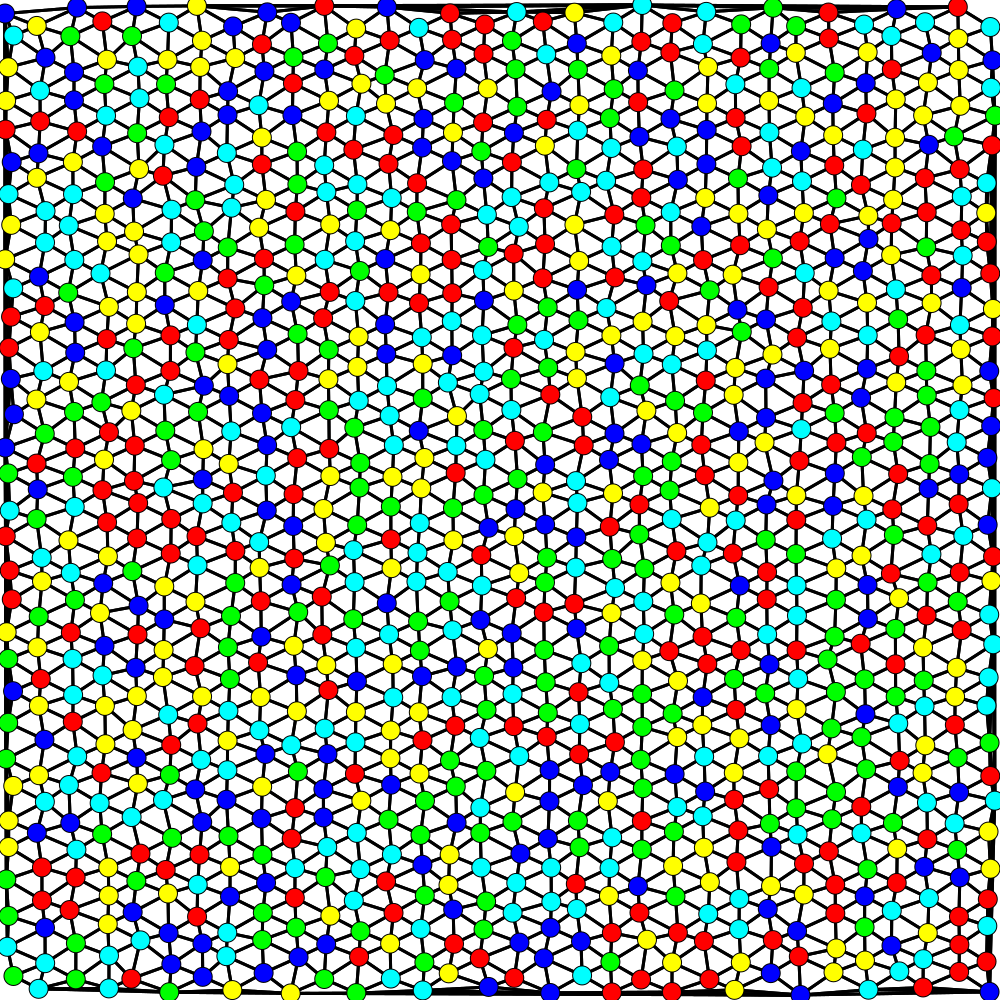
\includegraphics[width=\textwidth]{img/partitioning_false.png}
\caption{Non-partitioned graph.}
\end{subfigure}
~
\begin{subfigure}[b]{0.48\textwidth}
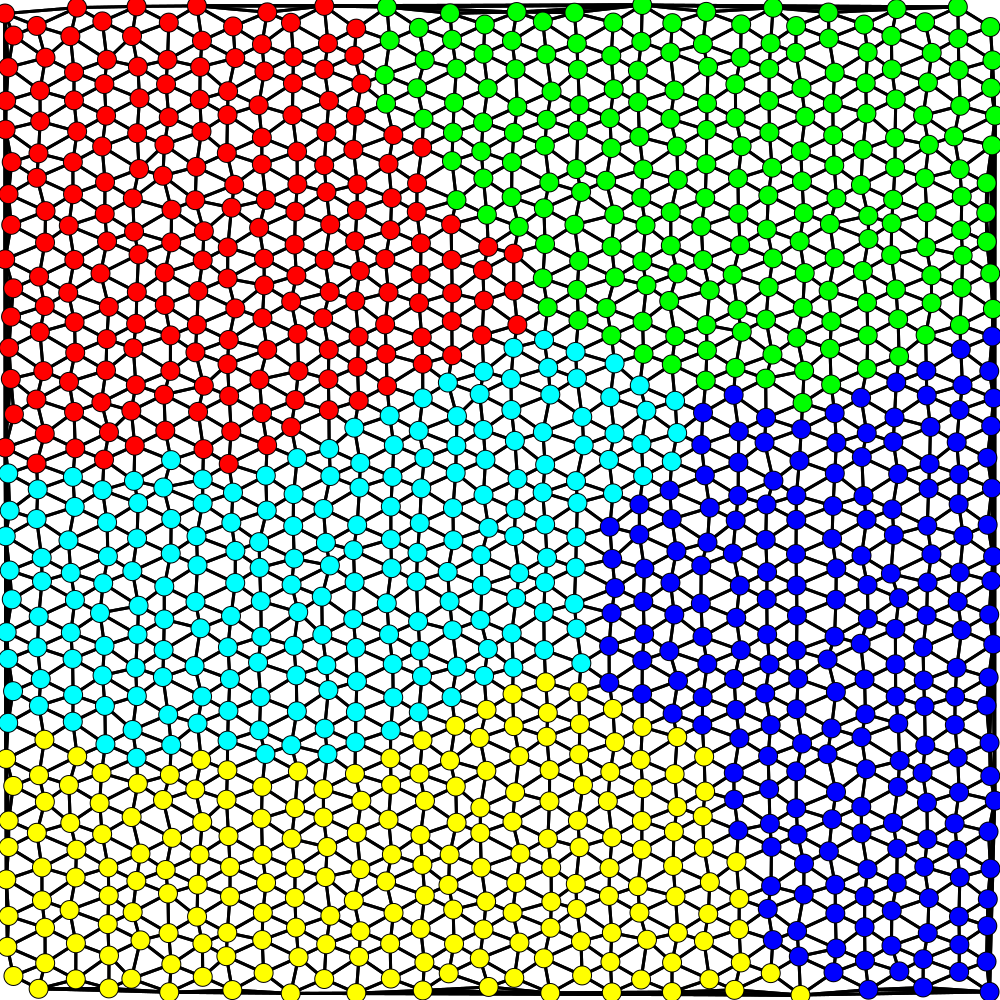
\includegraphics[width=\textwidth]{img/partitioning_true.png}
\caption{Partitioned graph.}
\end{subfigure}
\caption{Figure shows the difference in number of edges connecting nodes belonging to different cores for non-partitioned and partitioned graphs. Each colour represents nodes belonging to different cores. The partitioned graph was partitioned with METIS.}
\label{fig:partitioning}
\end{figure}

This method for increasing performance is applied in such a way that each core being used in the simulation is assigned a partition of the graph, hence the number of partitions and the number of cores must be equal. In both the preparation step and the confirmation step in Algorithm \ref{alg:outline} cache is invalidated since nodes write and read data that other nodes use. With the graphs partitioned a lot less cache is invalidated since the number of edges connecting nodes belonging to different cores are much smaller when each core handles a partition rather than nodes scattered all over the graph. The only cache that is invalidated now is the cache used by nodes laying on the boundary of the partitions.
